\chapter{Genomic Location Effect}\label{gle}

The tendency for mutations to occur in closed \gls{chromatin} regions has been reported both in cancer and other mutagenesis processes \citep{Polak2015,Prendergast2007ChromatinGenome}. This is hypothetically because closed chromatin regions, despite being less exposed to mutagens, are harder for repair systems to reach \citep{Prendergast2007ChromatinGenome,Teng1997ExcisionSequences, Morse2002PhotoreactivationCerevisiae}. Section \ref{gle:chromatin} of this chapter shows further evidence that mutations did tend to occur in closed rather than open chromatin regions. However, the influence of chromatin structure was not discriminative between cancers. Nevertheless, section \ref{gle:bootstrap} shows that \gls{gle} was significantly different between cancers. 

\section{Mutation location is influenced by chromatin status}\label{gle:chromatin}
My analyses of GLE were motivated observations that suggests mutations tend to locate in closed chromatin regions. Figure \ref{fig:mutation_density} shows the distribution of mutations on chromosome 12 for four cancers, the rest can be found in Figure \ref{fig:apdx_mutation_density} of the appendix. The shaded DHS bars near the bottom of the plots are hypersensitive regions (open chromatin) for the original cells, which was identified by literature search and shown in Table \ref{tab:encode}). The choice to display chromosome 12 was arbitrary. By visualisation alone, it can already be seen that mutation density was greater in less dense DHS, indicating a bias towards closed chromatin regions for the cancers of interest. This pattern was particularly strong in Skin-Melanoma and Liver-HCC, and less obvious in Kidney-RCC. It is also worth noting that the chromatin structures appeared different between cancers. Looking at the density by itself, we could see a diversity in how mutations are distributed, supporting the potential of GLE in discriminating cancers. 
% \newpage

\begin{figure}[ht!]
    \begin{subfigure}{.5\textwidth}
    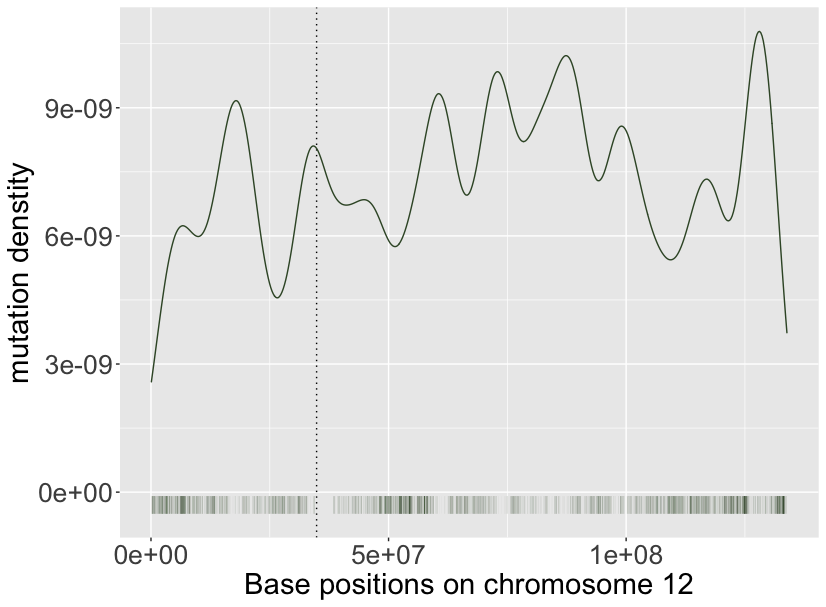
\includegraphics[width=\linewidth,height=0.7\textwidth]{graphics/mutdistribution_Skin-Melanoma.png}
    \caption{Skin-Melanoma}
    \label{fig:density_skin}
    \end{subfigure}
    ~
    \begin{subfigure}{.5\textwidth}
    
    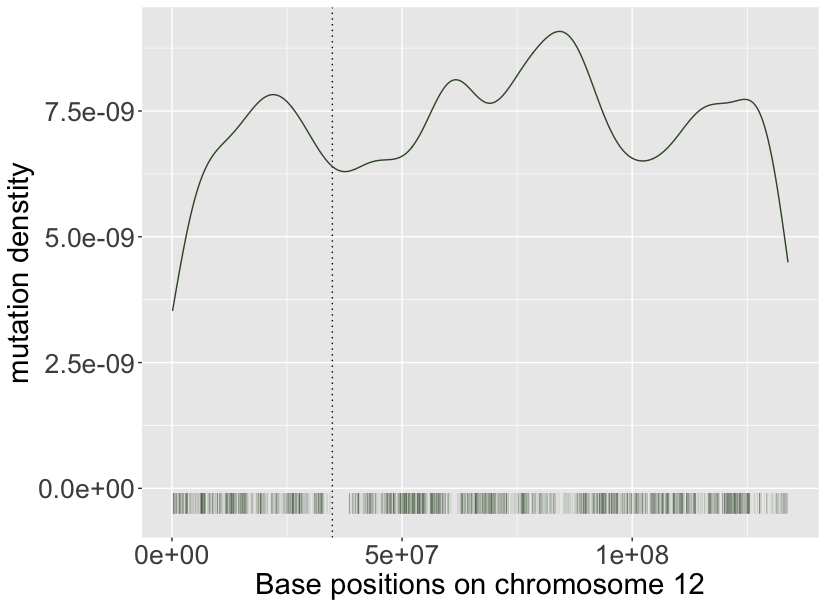
\includegraphics[width=\linewidth,height=0.7\textwidth]{graphics/mutdistribution_Kidney-RCC.png}
    \caption{Kidney-RCC}
    \label{fig:density_kidney}
    \end{subfigure} \\
    \vspace{0.5cm}
    
    \begin{subfigure}{.5\textwidth}
    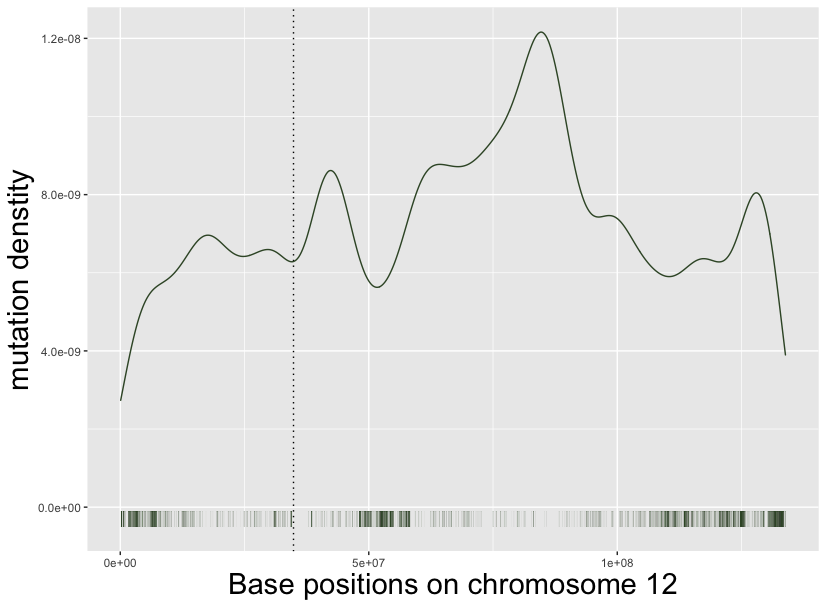
\includegraphics[width=\linewidth,height=0.7\textwidth]{graphics/mutdistribution_Liver-HCC.png}
    \caption{Liver-HCC}
    \label{fig:density_liver}
    \end{subfigure}
    ~
    \begin{subfigure}{.5\textwidth}
    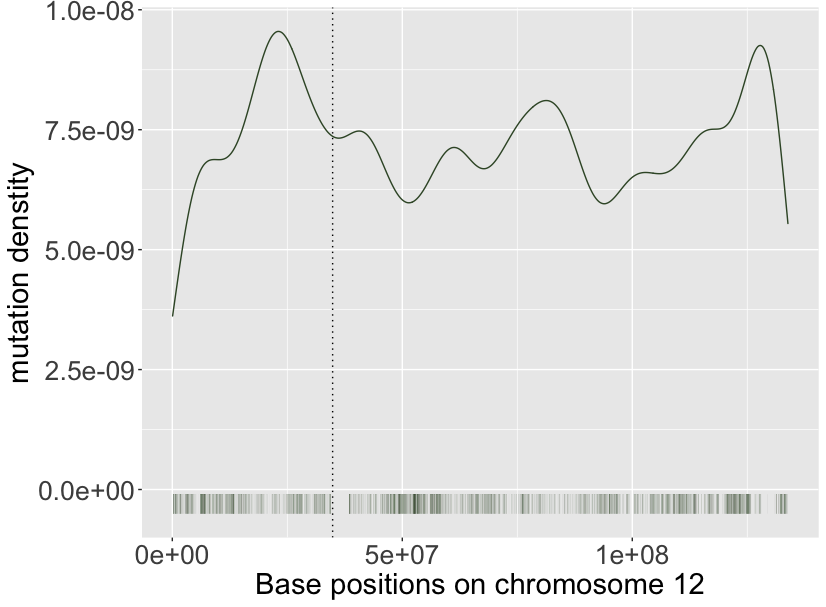
\includegraphics[width=\linewidth,height=0.7\textwidth]{graphics/mutdistribution_Panc-AdenoCA.png}
    \caption{Panc-AdenoCA}
    \label{fig:density_panc_adenoca}
    \end{subfigure} \\
    \caption{\textbf{Mutations tend to be found in closed chromatin regions.} Different cancers differ in the distribution of mutations across the genome. Here chromosome 12 is shown. (a) Skin-Melanoma (b) Kidney-RCC (c) Liver-HCC (d) Panc-AdenoCA, the other cancers are shown in Figure \ref{fig:apdx_mutation_density}. The shaded bars below the x-axis indicate open chromatin regions, the gaps indicate closed chromatin regions of the original cell types. The vertical dotted line indicates the position of the centromere.}
    \label{fig:mutation_density}
\end{figure}

\subsection{Some cancers were more similar than others in terms of chromatin structures}
In investigating whether the diversity in GLE is influenced by chromatin structure, one factor worth considering is how cancers relate to each other by the chromatin structure of their original cells to begin with. To compute the difference between the DHS of two original cell types, I identified the span of the intersection of their open chromatin regions and converted it into a distance (details in Methods \ref{methods:encode_pca}). The distance between every pair of cells allows calculating and visualising their relative coordinates using multidimensional scaling. Figure \ref{fig:encode_pca} shows the three most informative dimensions (PC1, PC2 and PC3) for the relationship between the original cells of cancers. Melanocyte and hepatocyte had the most distinct chromatin structures as they were relatively far away from the other cell types. On the other hand, prostate epithelium (ProstEpi) and exocrine cells of the pancreatic duct (PancDuct) were very close with respect to DHS on both panels of Figure \ref{fig:encode_pca}.

% \begin{figure}[h!]
%     \begin{subfigure}{.5\textwidth}
%     \centering
%     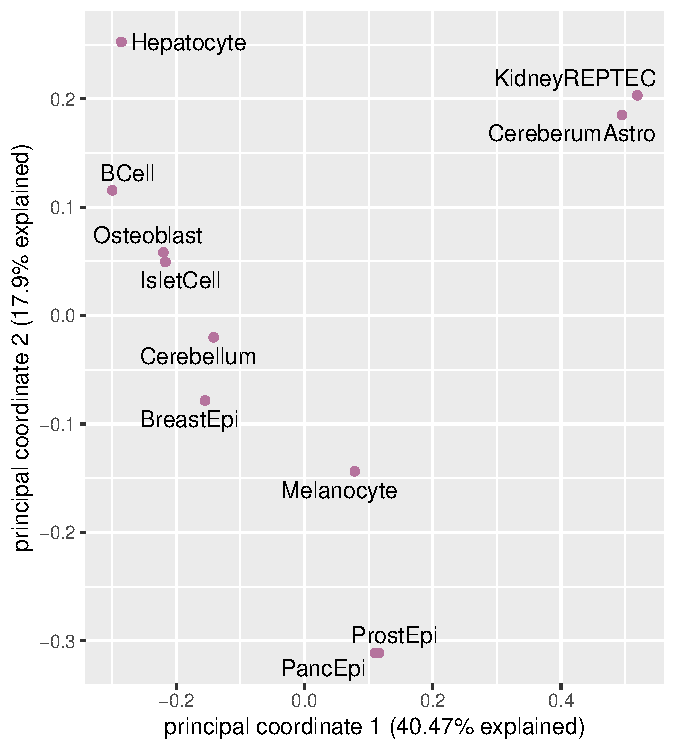
\includegraphics[scale=0.7]{graphics/encode_pca_1_2.pdf}
%     \caption{PC2 \textit{v.s.} PC1}
%     \end{subfigure}
%     ~
%     \begin{subfigure}{.5\textwidth}
%     \centering
%     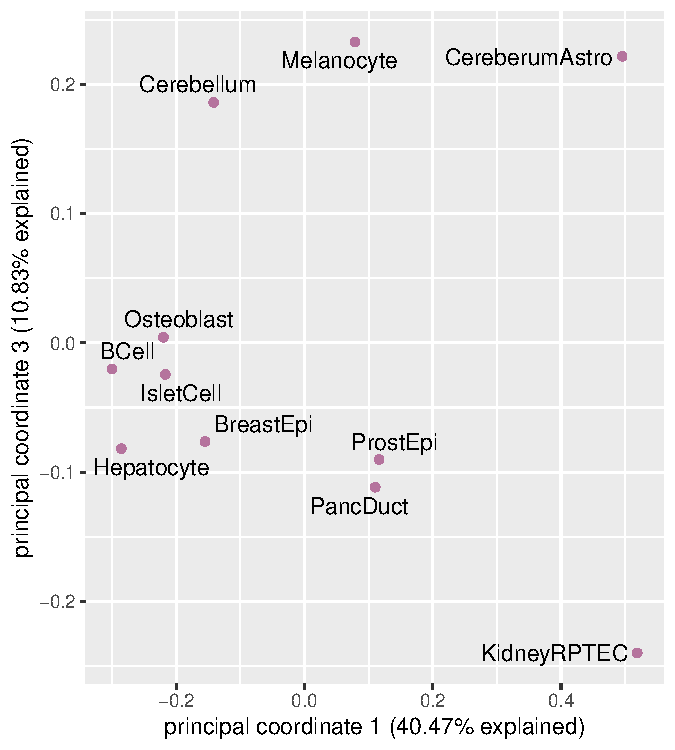
\includegraphics[scale=0.7]{graphics/encode_pca_1_3.pdf}
%     \caption{PC3 \textit{v.s.} PC1}
%     \end{subfigure} \\
%     \caption{\textbf{PCA}.}
%     \label{fig:encode_pca}
% \end{figure}

\begin{figure}[h!]
  \begin{minipage}[c]{\textwidth}
    \begin{subfigure}{.5\textwidth}
    \centering
    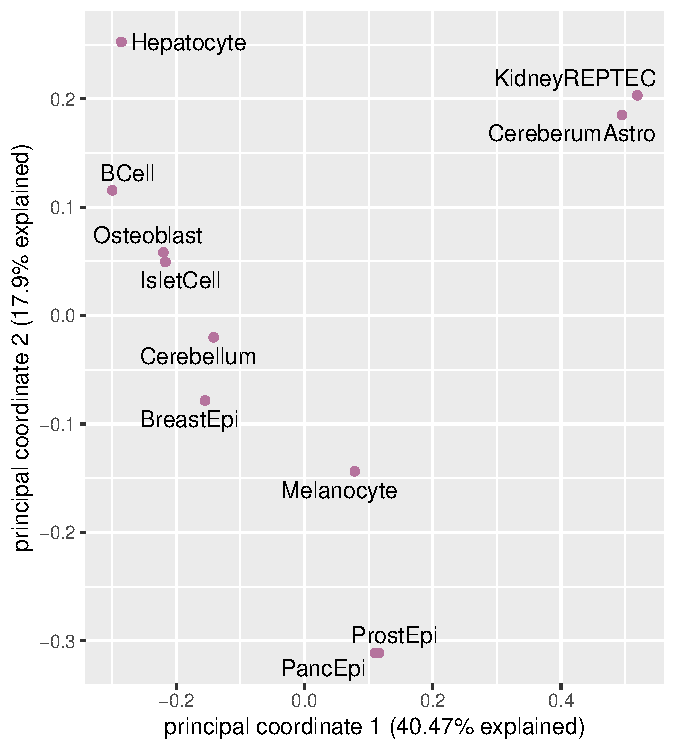
\includegraphics[scale=0.7]{graphics/encode_pca_1_2.pdf}
    \caption{PC2 \textit{v.s.} PC1}
    \end{subfigure}
    ~
    \begin{subfigure}{.5\textwidth}
    \centering
    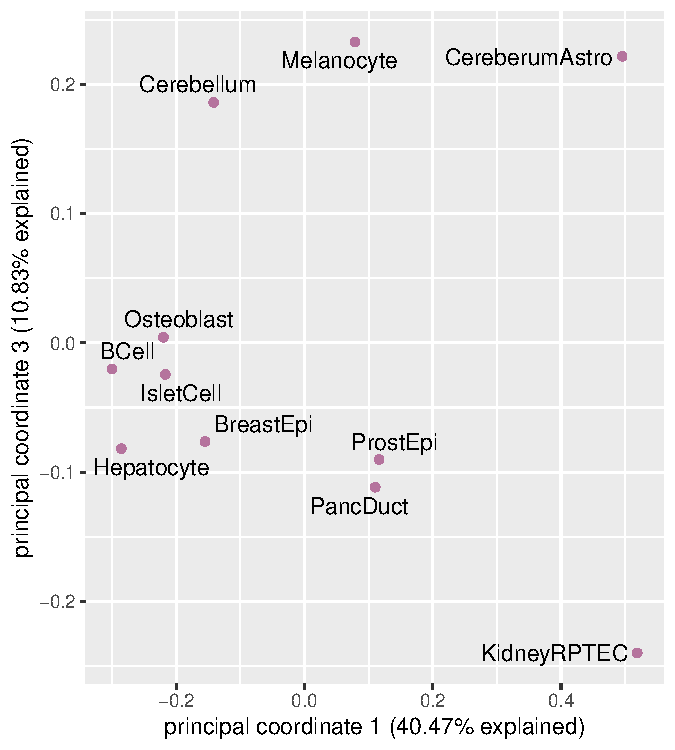
\includegraphics[scale=0.7]{graphics/encode_pca_1_3.pdf}
    \caption{PC3 \textit{v.s.} PC1}
    \end{subfigure} \\
  \end{minipage}\hfill
  \vspace{1cm}
  
  \begin{minipage}[c]{\textwidth}
    \centering
    \begin{tabulary}{\textwidth}{ ll }
    \toprule
    \textbf{Original cell abbreviation} & \bf{Cancer Type}  \\
    \toprule
    Osteoblast & Osteosarcoma \\
    
    BreastEpi & Breast-AdenoCa \\
    
    Cerebellum &  CNS-Medullo  \\
    
    CereberumAstro & CNS-PiloAstro \\
    
    KidneyRPTEC & Kidney-RCC \\
    
    Hepatocyte & Liver-HCC \\
    
    BCell & Lymph-BNHL, Lymph-CLL \\
    
    PancDuct & Panc-AdenoCa \\
    
    IsletCell & Panc-Endocrine \\
    
    ProstEpi & Prost-AdenoCa \\
    
    Melanocyte & Skin-Melanoma \\
    \bottomrule
    
    \end{tabulary}
    
    % . DHS data for these cells is downloaded from either \href{https://genome.ucsc.edu/cgi-bin/hgFileUi?db=hg19&g=wgEncodeOpenChromDnase}{Duke} or \href{https://genome.ucsc.edu/cgi-bin/hgFileUi?db=hg19&g=wgEncodeUwDnase}{UW} project
  \end{minipage}\hfill
  \vspace{0.5cm}
  
  \begin{minipage}[c]{\textwidth}
    \caption{
      \textbf{Some cancers were more related in terms of chromatin structures than others.} Here, I visualised the relative coordinates of the original cell types for cancers on the most informative dimensions (principle coordinates, PC). This was done by multidimensional scaling of the pairwise distance between cell types. The distance between two cell types was computed based on the intersection between their open chromatin regions. 
    } \label{fig:encode_pca}
  \end{minipage}
\end{figure}

\newpage

\subsection{Open and closed chromatin regions have significantly different mutation rates}
Having visualised the tendency of mutation location and the relationship between the chromatin structures of the original cells, I performed a hypothesis test to confirm whether there was a difference in how mutations are distributed between open and closed chromatin regions. This was achieved using the G-test of independence (details in Methods \ref{methods:chromatin}). The p-values obtained from this were adjusted using Bonferroni multiple test correction (Table \ref{tab:g-test}, the raw inputs can be found in Appendix \ref{apdx:g-test}). To begin with, the size of the regions identified as open chromatin is considerably tiny compared to that of closed chromatin regions. Keeping that in mind, we can see that most cancers had significantly different mutation rates between open and closed chromatin regions, except CNS-PiloAstro and Panc-Endocrine. Note that these two cancers had small to modest numbers of mutations. While no direct correlation between p-values and number of mutations could be detected, no cancers with less than 1 million mutations gave a p-value $>10^{-100}$. Our conclusion remains that mutation location is not random between open and closed chromatin regions, but this implies the impact of mutation load on the power of the test. 

% latex table generated in R 4.1.0 by xtable 1.8-4 package
% Tue Oct 19 08:53:20 2021
\begin{table}[h]
\centering
\caption{\textbf{The chance of mutations occurring are significantly different between closed and open regions for most cancers.} The table presents }
\label{tab:g-test}
\begin{tabular}{lrr}
  \toprule
 \textbf{Disease} & \textbf{$\hat{p}$-value} & \textbf{Number of mutations} \\ 
  \hline
 Bone-Osteosarc & 5.66 $\times 10^{-35}$ & 166845 \\ 
 Breast-AdenoCa & 1.33 $\times 10^{-10}$ & 713855 \\ 
 CNS-Medullo & 2.46 $\times 10^{-34}$ & 209997 \\ 
 CNS-PiloAstro & 1.00 & 22020 \\ 
 Kidney-RCC & 2.60 $\times 10^{-06}$ & 531886 \\ 
 Liver-HCC & $<10^{-100}$ & 3321521 \\ 
 Lymph-BNHL & $<10^{-100}$ & 1124881 \\ 
 Lymph-CLL & $<10^{-100}$ & 226242 \\ 
 Panc-AdenoCA & $<10^{-100}$ & 1675781 \\ 
 Panc-Endocrine & 8.82 $\times 10^{-02}$ & 258564 \\ 
 Prost-AdenoCA & 5.49 $\times 10^{-90}$ & 1000496 \\ 
 Skin-Melanoma & $<10^{-100}$ & 7770980 \\ 
   \bottomrule
\end{tabular}
\end{table}

\subsection{Mutations were typically biased towards closed regions}
Complementary to the G-tests, which suggested that the difference in mutation location were statistically significance between closed and open chromatin regions, I computed the odds ratio ($OR$), which measures the direction of this difference. From equation \ref{eq:or}, $OR$ compares the ratios of mutated over non-mutated positions between closed and open regions. An $OR>1$ indicates a bias towards closed regions, and an $OR<1$ indicates a bias towards open regions. For each cancer, I estimated the standard error of $OR$'s using jackknife, where one donor was removed to obtain a pseudo-$OR$. The standard errors of the resulting pseudo-$OR$'s were the jackknifed standard error for $OR$. The results are shown in Figure \ref{fig:or_jackknifed}.

\begin{figure}[h!]
    \centering
    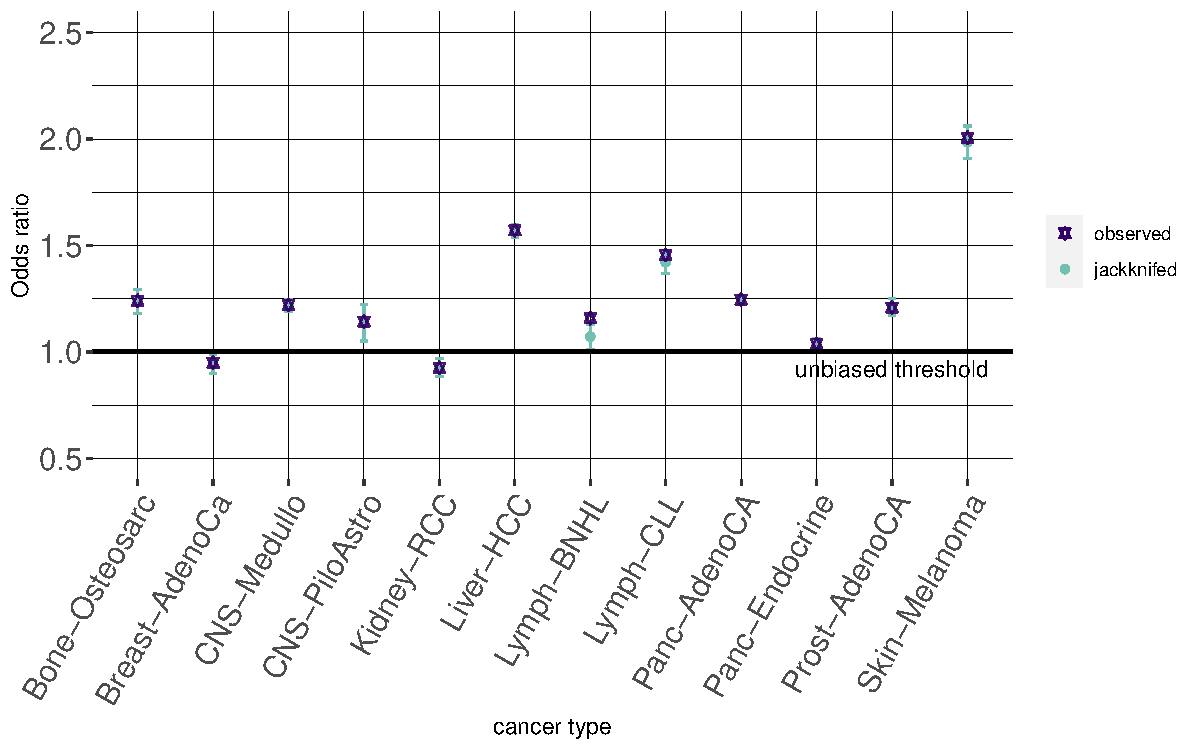
\includegraphics[scale=0.8]{graphics/jackknife_OR.pdf}
    \caption{\textbf{Mutations tend to occur in closed chromatin regions according to the odds ratio ($OR$) statistic}. $OR>1$ indicates a bias towards towards closed regions, and $OR<1$ indicates the opposite. Error bars are the standard errors of the jackknifed sample. The green circles are the means of the jackknifed pseudo-values. The purple stars are the observed $OR$.}
    \label{fig:or_jackknifed}
\end{figure}


Overall, mutations preferred to locate in closed chromatin regions, especially for Skin-Melanoma ($OR=2$). However, this bias varied between cancers. In addition, there are three other intriguing features. First, Breast-AdenoCa and Kidney-RCC had $OR<1$. Their p-values from the G-test showed a significant difference between closed and open regions, suggesting that the preference for open regions was not due to noise. On the density plot (Figures \ref{fig:mutation_density} and \ref{fig:apdx_mutation_density}), mutations still peaked at closed chromatin regions, but less clear than for example Skin-Melanoma. Second, the departure of the observed $OR$ from the mean pseudo-values in Lymph-BNHL and Lymph-CLL suggests an abnormality in these cases. This abnormality could be due to the large variance of GLE in donors with these cancers. However, it could also come from the uncertainty in identification of the original cells (B cells for both cancers, discussed in \ref{}). Third, CNS-PiloAstro had the largest standard error of $OR$. Again, this might be because its small number of mutations lowered the signal to noise ratio compared to other cancers, which is consistent with the G-test results. Regarding reliability, empirically, $OR$ seems more robust to the number of mutations than G-test. Mathematically, it accounts for the imbalance in the size of open \textit{v.s.} closed chromatin regions. However, we need to be vigilant about the existence of this imbalance.

\subsection{Chromatin structure was influential but not discriminative}

In this subsection, I evaluated the appropriateness of $OR$ given the imbalance between the size of open and closed chromatin regions and the potential of $OR$ in discriminating cancers. The evaluation was done by calculating the $OR$'s with mislabelled DHS data. That is, I sorted a cancer's mutation data based on other cancers' DHS data rather than its own (Methods \ref{methods:chromatin}). 

The impact of imbalanced DHS was assessed in Figure \ref{fig:mixed_or_violin}. Specifically, I examined whether the very large size of closed chromatin regions rather than its biological properties made mutations in closed regions more likely. If $OR$ was sensitive to the imbalance, then each violin should have had a distinctive value. A good example to illustrate this involves Skin-Melanoma and Kidney-RCC, whose ratios of closed over open chromatin regions were 65 and 115 in their original cells' DHS, respectively (Table \ref{fig:tab_g-test_contingency}). If $OR$ was sensitive, then it should have always been higher in Kidney-RCC than Skin-Melanoma, no matter what mutation data was used. This was not the case. $OR$ range was approximately the same for Kidney-RCC and Skin-Melanoma, which suggests that the effect of the imbalance in DHS data was mild.

However, it is curious that $OR$ was not typically the highest when DHS data of the true cancer was used. This was further reinforced in Figure \ref{fig:mixed_or_heatmap}. Each column of Figure \ref{fig:mixed_or_heatmap}, representing a cancer whose DHS data was used, was coloured with respect to the rank of $OR$'s for cancers with mutation data. It is worth noting that Figure \ref{fig:mixed_or_violin} is basically the violin plot by the columns of Figure \ref{fig:mixed_or_heatmap}, where each violin contains the $OR$'s with mislabelled mutation data and a fixed DHS data. Mutation data for Skin-Melanoma almost always produced one of the highest $OR$'s, irrespective of the cancer types used for DHS data. Another way to view this is to use the violin plot by the rows rather than columns of the heatmap, where DHS data is mislabelled (Figure \ref{fig:mixed_or_byrow}). Contrary to plotting $OR$ against mislabelled mutation data (DHS data being the determinant), plotting $OR$ against mislabelled DHS data (mutation data being the determinant) showed distinctive ranges of $OR$ for most cancers, except Liver-HCC. This means that $OR$ was determined by the properties of mutation data instead of DHS data. Accordingly, chromatin structure, in the form of $OR$ is indicative of mutation location, but it is unlikely to be the main determinant of whether GLE differs between cancers. One possible explanation is the similarities in the DHS data of the original cells.

\begin{figure}[ht!]
    \begin{subfigure}{\textwidth}
    \centering
    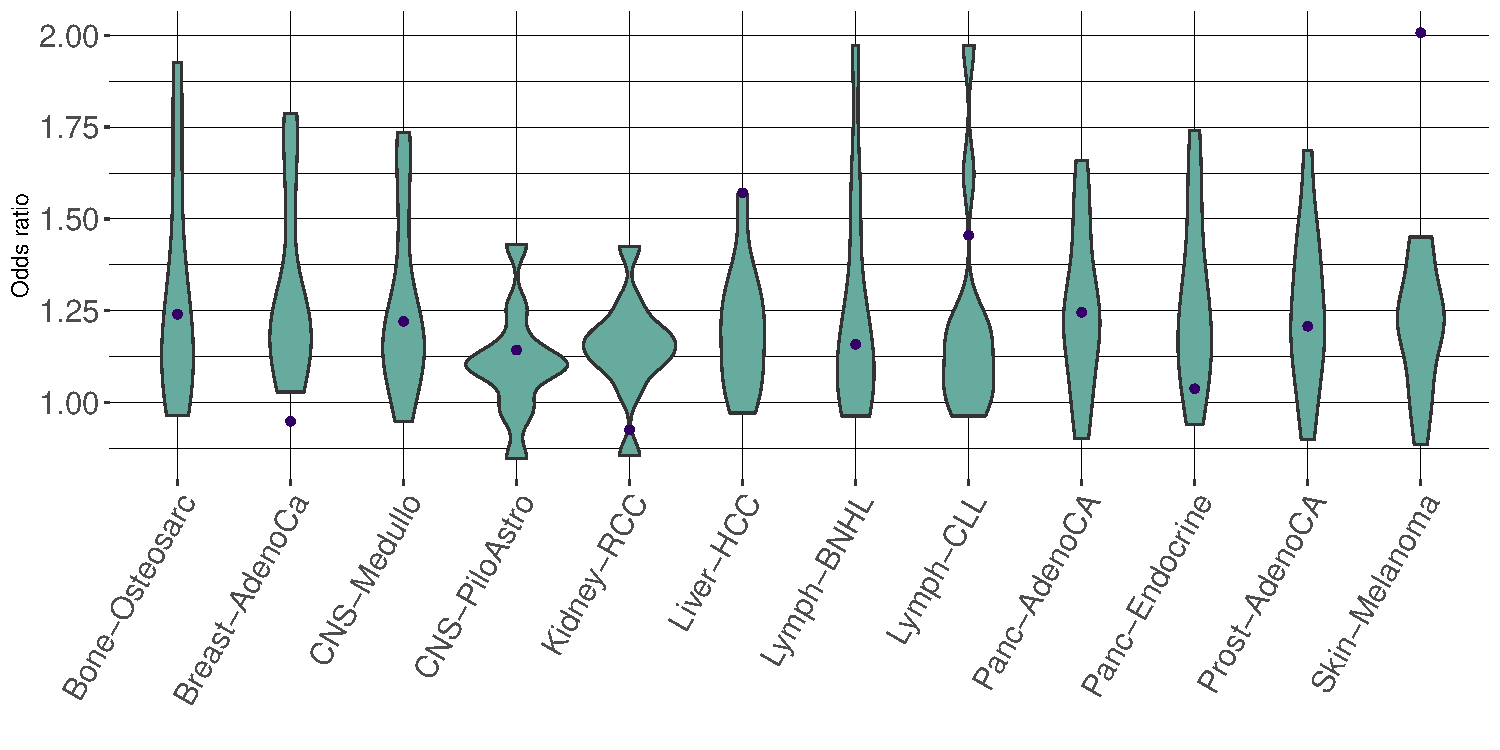
\includegraphics[scale=0.5]{graphics/mixed_or_violin.pdf}
    \caption{The impact of imbalanced DHS data on $OR$ is mild}
    \label{fig:mixed_or_violin}
    \end{subfigure} \\
    
    \vspace{0.3cm}
    \begin{subfigure}{\textwidth}
    \centering
    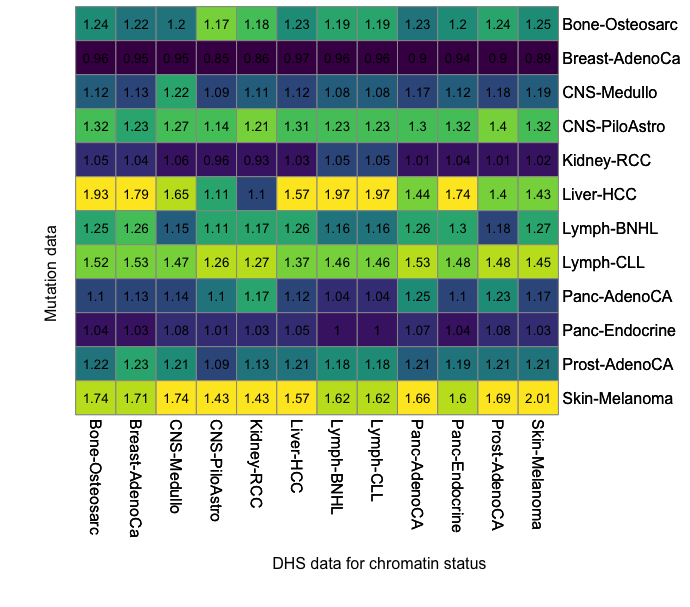
\includegraphics[scale=0.52]{graphics/mixed_or_heatmap.png}
    \caption{Chromatin structure is not discriminative of cancers}
    \label{fig:mixed_or_heatmap}
    \end{subfigure} 
\caption{}
    % \caption{\textbf{(a) The bias of mutations towards closed regions was not due to their large size compared to open regions but (b) this bias was unlikely the reason why GLE differs between cancers.} This figure shows an experiment where $OR$'s were calculated by cross-matching DHS data with mutation data of different cancers. In (a), the x-axis is the cancers whose DHS data was used, the y-axis is the distribution of $OR$ with mislabelled mutation data, with the purple dot indicating when mutation data of the correctly labelled cancer was used. In (b), the column labels are the cancers whose DHS data was used, the row labels are the cancers whose mutation data was used; each column is coloured by the rank of $OR$'s, brighter colours come from cancers whose mutation data produced the greater $OR$'s.}
    \label{fig:mixed_or}
\end{figure}

\section{GLE is significantly different for different cancers}\label{gle:bootstrap}
Previously, we observed different patterns of GLE for different cancers by visualisation (Figure \ref{fig:mutation_density}). In this section, I investigated whether the difference is statistically significant and what data representations are optimal for GLE. For each pair of cancers, I used a bootstrap hypothesis test for whether their GLE are significantly different. I trialled two representations (bin and smoothing) and two distance measures (Euclidean and Wasserstein) to see which representation/measure could best discriminate cancers. I reported the raw p-values rather than recruiting multiple test correction because if two reasons. First, the true purpose of this section was to detect signals in the data, so it was not particularly meaningful to set a rigid significance threshold. Second, each p-value was estimated from 1000 simulations of a cancer pair; consequently, the p-values obtained were not drawn from the same distribution. From Table \ref{tab:gle_bootstrap}, GLE was generally very different for all cancer pairs. The smoothing representation were more likely to output more significant p-values, with only two pairs at p-values $>0.001$ for Wasserstein and no pairs for Euclidean distance. The most common cancer with p-value $>0.001$ was CNS-PiloAstro, which might be due to its small sample size, as in the case with the G-test and the $OR$. 

\begin{table}[!htb]
    \caption{\textbf{Estimated p-values from bootstrap hypothesis tests involving 1000 simulations for (a) Bin/Euclidean, (b) Bin/Wasserstein, (c) Smooth/Euclidean, (d) Smooth/Wasserstein} No multiple test correction was applied. All estimated p-values were $<0.001$ unless otherwise specified.}
    \label{tab:gle_bootstrap}
    % row 1
    \begin{subtable}[!h]{.5\textwidth}
        \centering
        \begin{tabular}{ p{3cm}p{2.7cm}c }
        & \textbf{CNS-PiloAstro} & \textbf{others} \\
        \textbf{CNS-Medullo} & 0.121 & - \\
        \textbf{Kidney-RCC} & 0.024 & - \\
        \textbf{Liver-HCC} & 0.121 & - \\
        \textbf{Panc-Endocrine} & 0.069 & - \\
        \textbf{Prost-AdenoCA} & 0.009 & - \\
        \textbf{all others} & - & - \\
        \end{tabular}
        \vspace{0.2cm}
    \subcaption{Bin/Euclidean}
    \end{subtable} 
    \quad % for side by side tables
    \begin{subtable}[!h]{.5\textwidth}
        \centering
        \begin{tabular}{ p{2.9cm}p{2.7cm}c }
        & \textbf{CNS-PiloAstro} & \textbf{others} \\
        \textbf{Bone-Osteosarc} & 0.034 & - \\
        \textbf{Panc-AdenoCA} & 0.024 & - \\
        \textbf{Skin-Melanoma} & 0.017 & - \\
         &  &  \\
         &  &  \\
        \textbf{all others} & - & - \\
        \end{tabular}
        \vspace{0.2cm}
    \subcaption{Bin/Wasserstein}
    \end{subtable}  
    % row 2
    \begin{subtable}[!h]{.5\textwidth}
        \centering
        \begin{tabular}{ p{3cm}p{2.7cm}c }
        &  & \textbf{All} \\
        &  &  \\
        &  &  \\
        \textbf{All} & - & - \\
        \end{tabular}
        \vspace{0.2cm}
    \subcaption{Smooth/Euclidean}
    \end{subtable} 
    \quad % for side by side tables
    \begin{subtable}[!h]{.5\textwidth}
        \centering
        \begin{tabular}{ p{2.9cm}p{2.7cm}c }
        & \textbf{CNS-PiloAstro} & \textbf{others} \\
        \textbf{Panc-AdenoCA} & 0.005 & - \\
        \textbf{Prost-AdenoCA} & 0.031 & - \\
        \textbf{all others} & - & - \\
        \end{tabular}
        \vspace{0.2cm}
    \subcaption{Smooth/Wasserstein}
    \end{subtable}  
    
\end{table}


